\documentclass[12pt]{article}
\usepackage[a4paper, margin=.30in]{geometry}
\usepackage{graphicx ,
            wrapfig,
            xcolor, 
            enumerate,
            amsmath,fontenc,tcolorbox
            }
\usepackage[european, straightvoltages,EFvoltages]{circuitikz}
\newcommand\headerMe[2]{\noindent{}#1\hfill#2}
\renewcommand{\thesection}{\Roman{section}}

\title{Leçon : }
\author{Zakaria HAOUZAN}
\date{\today}

\begin{document}
% headers --------------
\headerMe{Matière : Physique-Chimie}{Professeur : Zakaria HAOUZAN}\\
\headerMe{Unité : La Mécanique}{Établissement : Lycée SKHOR qualifiant}\\
\headerMe{Niveau : TCS}{Heure : 2H}\\

% ------Content ________
\begin{center}
  \Large{Leçon $N^{\circ}12$: \color{red} Caractéristique d'un dipôle actif}
\end{center}

\section{Dipôles actifs : }

\subsection{Définition:}
Un dipôle est dite actif si, en circuit ouvert, la tension à ses bornes n’est pas nulle.

Exemples : Piles, accumulateurs.
%\begin{wrapfigure}[4]{r}{0.39\textwidth}
    %\vspace{-1cm}
%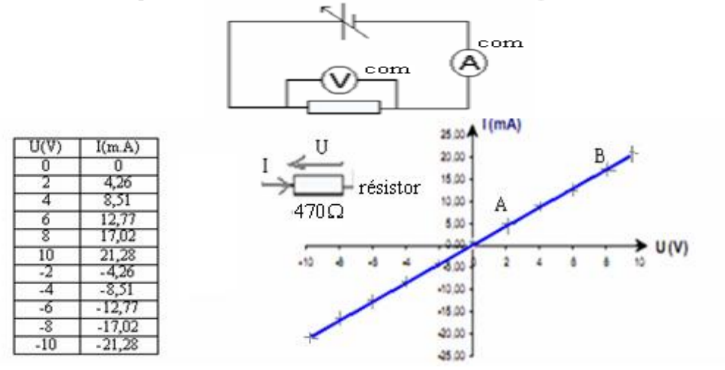
\includegraphics[width=0.39\textwidth]{./img/caracteristique_Resistor.png}
%\end{wrapfigure}


\subsection{Convention générateur }

Dans la convention récepteur la tension U aux bornes d'un dipôle passif et l'intensité I du courant qui le traverse
sont de sens contraires.


\begin{center}
  \begin{circuitikz}[european resistors]
    \draw (-0.5,0.1)node{A} (0,0)to[battery1=$\,$,v=$U_{AB}$,i>=I, name=D] (2,0);
      \draw (2.2, 0) node{B};
    
  \end{circuitikz}
  \end{center}

\section{Caractéristique d’un dipôle actif }
\subsection{ Définition :}
On appelle graphe caractéristique d’un dipôle actif le graphe de la fonction qui lie la tension UPN entre ses bornes au courant I qui le traverse.
\begin{wrapfigure}[5]{r}{0.39\textwidth}
\begin{center}
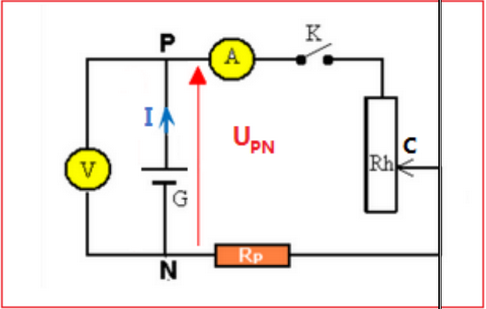
\includegraphics[width=0.39\textwidth]{./img/Pile_use.png}
\end{center}
\end{wrapfigure}

\subsection{Caractéristique d’une pile}
\subsubsection{Montage électrique :}
L’interrupteur K est ouvert on mesure la tension UPN.
On ferme K et on déplace le curseur C le long du
rhéostat, on relève les valeurs de UPNet I on obtient le
tableau suivant :

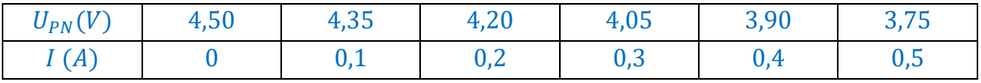
\includegraphics[width=0.5\textwidth]{./img/table.png}
%\end{center}

\begin{wrapfigure}[12]{r}{0.39\textwidth}
\begin{center}
  \vspace{-1.7cm}
  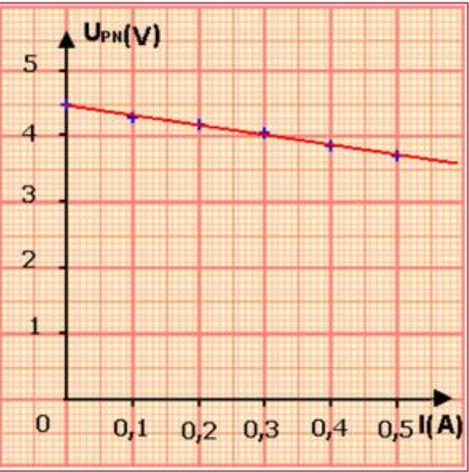
\includegraphics[width=0.39\textwidth]{./img/tension_courant.png}
\end{center}
\end{wrapfigure}
\subsubsection{ la caractéristique intensité du
courant-tension}
La caractéristique est une droite qui ne passe pas
par l’origine, il représente une fonction affine
d’équation : $U_{PN} = aI + b$.

La valeur de a : Le coefficient directeur a est négatif et s’exprime
en $V.A^{-1}$ c’est-à-dire en ohm. 

a est l’opposé de la résistance a = -r, r est
appelé la résistance interne du générateur. $$r = \lvert{a}\rvert=> r = \lvert\frac{\Delta{U_{PN}}}{\Delta{I}}\rvert = \lvert\frac{4.50-3.75}{0-0.5}\rvert= 1.5\Omega$$

La valeur de b :
L’ordonné à l’origine b s’exprime en volt, il a les dimensions de la tension. b b= E.
E est appelé la force électromotrice du générateur. $b = E = 4.5V$

L’équation de la caractéristique de générateur : $U_{PN} = 4.5 - 1.5I$

\begin{tcolorbox}{La loi d’ohm pour le générateur : }
  $$U_{PN} = E - rI$$

  UPN:tension aux bornes du générateur en(V)

  E: force électromotrice du générateur en (V)

  r: résistance interne du générateur en ($\Omega$)

I:Intensité du courant qui traverse le générateur en (A)
\end{tcolorbox}
\begin{wrapfigure}[6]{r}{0.3\textwidth}
\begin{center}
  \vspace{-2.6cm}
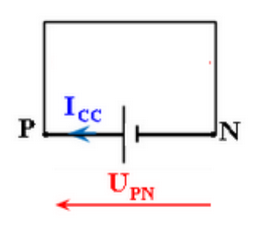
\includegraphics[width=0.2\textwidth]{./img/Icc_montage.png}
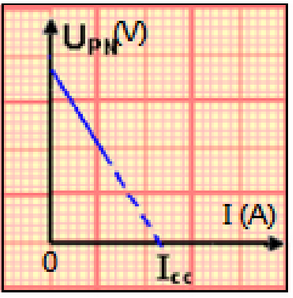
\includegraphics[width=0.19\textwidth]{./img/Icc_carca.png}
\end{center}
\end{wrapfigure}

\subsection{Intensité de court-circuit d’un générateur :}
Pour mettre le générateur en court-circuit, on relie ses pôles par un fil métallique, dans ce cas
la tension UPN est nulle.
$E - rI_{CC} = 0$ donc $I_{CC} = \frac{E}{r}$

\begin{tcolorbox}{Remarque :}
  
Un dipôle actif est idéal si sa résistance interne est
nulle ( r = 0).
\end{tcolorbox}
\subsection{Association en série des dipôles actifs linéaires : }
Soit deux piles G1(E1, r1) et G2
(E2, r2 ) associées en série, cette association est équivalente à un dipôle actif G(E, r).

\begin{center}
  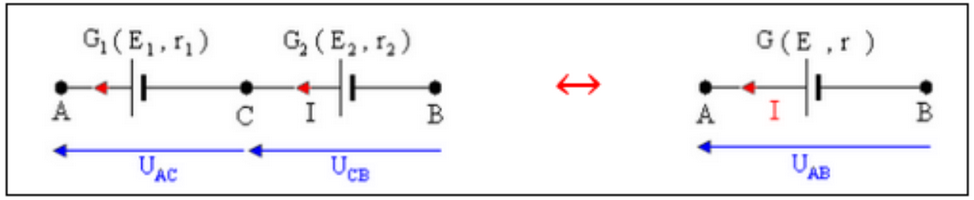
\includegraphics[width=0.5\textwidth]{./img/sum_gene.png}
\end{center}
D’après la loi d’additivité des tensions : $U_{AB} = U_{AC} + U_{CB}$
La loi d’ohm pour les trois piles : $U_{AC} = E_1 - r_1I$ ; $U_{BC} = E_2 - r_2I$ ; $U_{AB} = E - rI$

donc $E = E_1 + E_2$ et $r = r_1 + r_2$

\begin{tcolorbox}{Généralisation }
L’association des n dipôles actifs et linéaires est équivalente à un dipôle actif et linéaire sa
force électromotrice : $E = \sum E_i$ et de résistance interne : $r = \sum r_i$
\end{tcolorbox}

\section{ Caractéristiques d’un récepteur (l’électrolyseur) :}
\subsection{ Définition :}
Un récepteur est un dipôle électrique qui convertit une partie d’énergie électrique qu’il reçoit
en une autre forme d’énergie autre que l’énergie thermique.

Exemples : un moteur, un électrolyseur.

\subsection{Convention récepteur :}
Dans la convention récepteur la tension $U_{AB}$ et l’intensité du courant I sont orientées dans le
sens contraires.

\begin{center}
  \begin{circuitikz}[european resistors]
    \draw (-0.5,0.1)node{A} (0,0)to[R,v=$U_{AB}$,i>=I, name=D] (2,0);
      \draw (2.2, 0) node{B};
    
  \end{circuitikz}
  \end{center}

\begin{wrapfigure}[4]{r}{0.3\textwidth}
\begin{center}
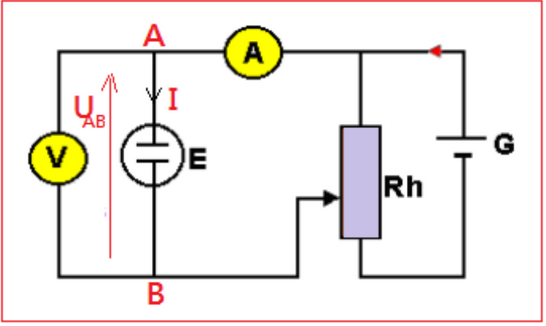
\includegraphics[width=0.3\textwidth]{./img/recepteur_mon.png}
\end{center}
\end{wrapfigure}



\subsection{Caractéristique de l’électrolyseur :}
\subsubsection{Montage expérimental : }
On déplace le curseur le long du rhéostat, on
relève les valeurs de UAB et de I .
\subsubsection{Tableau des résultats :}
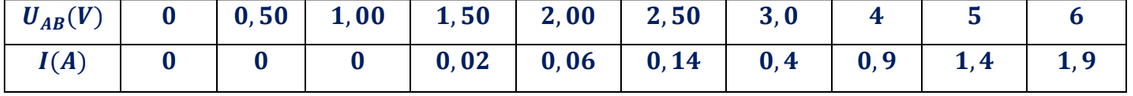
\includegraphics[width=0.7\textwidth]{./img/table_recep.png}


\begin{wrapfigure}[4]{r}{0.3\textwidth}
\begin{center}
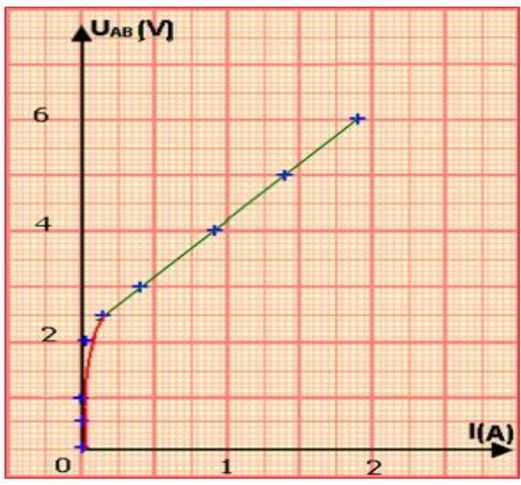
\includegraphics[width=0.3\textwidth]{./img/recep_carcater.png}
\end{center}
\end{wrapfigure}



\subsubsection{Caractéristique UAB = f(I) :}
La caractéristique intensité-tension de l’électrolyseur est une portion de droite d’équation :
$$U_{AB} = E' + r'I$$
E': force contre - électroomotrice (f. c. é. m)en (V)

r': résistance interne de l'électrolyseur en ($\Omega$)

$U_{AB}$:la tension aux brnes de l'électrolyseur en (V)

$E' = 2.2V$ et $r' = 2\Omega$

\begin{wrapfigure}[16]{r}{0.4\textwidth}
\begin{center}
  \vspace{-2cm}
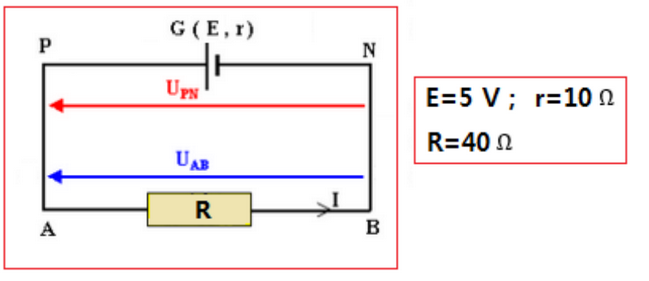
\includegraphics[width=0.4\textwidth]{./img/Montage_12.png}
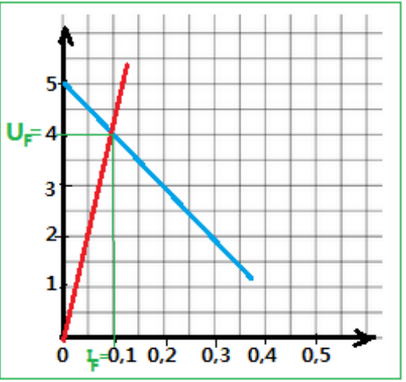
\includegraphics[width=0.4\textwidth]{./img/fonct_point.png}
\end{center}
\end{wrapfigure}


\section{Point de fonctionnement :}
\subsection{Notion de point de fonctionnement :}
Le branchement d’un dipôle actif (piles) aux bornes d’un dipôle passif (électrolyseur), forme un circuit électrique.

L’intensité $I_f$ du courant qui traverse le circuit et la tension Uf aux bornes du dipôle actif définit le point du fonctionnement du circuit $F(I_f ,U_f)$.
\subsection{Détermination du point du fonctionnement du circuit :}
\subsubsection{Méthode graphique :}
Traçant les caractéristiques de la pile et de conducteur ohmique dans le même repère.
Les deux caractéristiques se
coupent en un point F de
cordonnées : F$(I_f = 0, 1 A , U_f = 4 V )$
\subsubsection{ Méthode algébrique :}
Appliquant la loi d’ohm : Pour un générateur : UPN = E - r. I et Pour un conducteur ohmique : UAB = R. I

D’après la loi d’additivité des tensions : $U_{PN} = U_{AB}$
 donc $E-rI = R.I$
 alors $I = I_F = \frac{E}{R + r} = \frac{5}{50} = 0.1A$

\subsection{Loi de Pouillet : }

-On considère le montage qui contient :
Un générateur (E, r), un moteur $(E', r')$ et un conducteur ohmique de résistance R.

-Trouvons l’intensité du courant I qui circule dans le
circuit :

Appliquant la Loi d’ohm : UPN = E - r. I  Pour le générateur

$U_{AB}$ = E'+ r'. I Pour le moteur

$U_{BC}$ = R. I Pour le conducteur ohmique

D’après la Loi d’additivité des tensions : $I = \frac{E - E'}{R + r + r'}$ (1)

La relation (1) exprime la loi de Pouillet, qui concerne les circuits électriques constitués uniquement des dipôles linéaires associés en série.

\begin{tcolorbox}{Généralisation :} 
L’intensité du courant qui passe dans un circuit série comportant n générateurs, m récepteurs
  actifs et k conducteurs ohmiques est :$$I = \frac{\sum E_i - \sum E'_i}{\sum r_i + \sum r'_i + \sum R_i}$$
\end{tcolorbox}


\end{document}
